\documentclass{js}
\usepackage[dvipdfmx]{graphicx}
%\usepackage{latexsym}
\usepackage{txfonts}
%\usepackage[fleqn]{amsmath}
%\usepackage[psamsfonts]{amssymb}
%\usepackage[deluxe]{otf}
\usepackage{comment}

% 印刷位置調整 %
% 必要に応じて値を変更してください.
\hoffset -10mm % <-- 左に 10mm 移動
\voffset -10mm % <-- 上に 10mm 移動

\newcommand{\AmSLaTeX}{%
 $\mathcal A$\lower.4ex\hbox{$\!\mathcal M\!$}$\mathcal S$-\LaTeX}
\newcommand{\PS}{{\scshape Post\-Script}}
\def\BibTeX{{\rmfamily B\kern-.05em{\scshape i\kern-.025em b}\kern-.08em
 T\kern-.1667em\lower.7ex\hbox{E}\kern-.125em X}}

% \papernumber{DEIM Forum 2014 F1-6}

\jtitle{講義プレゼンテーションスライド部分対応付けを用いた学習支援}
%\jsubtitle{サブタイトル}
\authorlist{%
 \authorentry[sakamoto@db.soc.i.kyoto-u.ac.jp]{坂本 祥之}{Yoshiyuki SAKAMOTO}{kyotou}% 
 \authorentry[tshimizu@i.kyoto-u.ac.jp]{清水 敏之}{Toshiyuki SHIMIZU}{kyotou}% 
 \authorentry[yoshikawa@i.kyoto-u.ac.jp]{吉川 正俊}{Masastoshi YOSHIKAWA}{kyotou}% 
}
\affiliate[kyotou]{京都大学大学院情報学研究科}
 {}


%\MailAddress{$\dagger$hanako@deim.ac.jp,
% $\dagger\dagger$\{taro,jiro\}@jforum.co.jp}

\begin{document}
\pagestyle{empty}
\maketitle










\section{はじめに}

近年,学会での発表や講義などでプレゼンテーションスライドが使われることが増えている.
その中でも講義のスライドは,講義の復習のためや,学外の人のために,OCW(Open Course Ware)で公開されていることがある.
これらの講義スライドは,同様の話題が書かれたものでも,大学や講義によって記述の平易さや詳細さが異なる.
本研究では,まず,スライドをセグメントに分割し,異なるスライド間で類似したセグメントの対応付けを求める.
そして,この対応付けをもとに,閲覧者が現在閲覧している講義スライドに対して別のスライドを提示することで,講義スライド閲覧者の理解支援を行うことを考えている.

% \begin{verbatim}
%  \papernumber{DEIM Forum 2014 XX-Y}
% \end{verbatim}









\begin{comment}
\section{関連研究}

プレゼンテーションスライドからの情報取得や,検索等についての関連研究として,以下の研究が挙げられる.

羽山ら\cite{hayama2008} \cite{hayama2009}の研究では,1枚のスライド内の構造化を行なっている.
スライド内の配置の情報とフォントの情報から,スライド内のオブジェクトを,タイトル,本文,図,表,装飾という5つに分類し,一枚のスライド内の情報を木構造で表現している.

さらに,羽山らの別の研究\cite{hayama2010}は,\cite{hayama2009}の手法をベースとして,検索要求に関連する箇所だけを抽出し,提示する手法を提案している.

北山ら\cite{kitayama2009}の研究では,スライド間の関係を求めている.
この研究では,スライドの単語と,そのインデントの情報,発表テキストをデータとして利用している.
スライド間の関係としては,詳細化,汎化,具体化,付加の4種類を定義している.
ある基点スライドを決め,そのスライドに出現している一つの単語着目し,基点スライドと関係のあるスライドを求め,関係を分類している.
基点スライドが同じでも,着目する単語が違うと,関係が異なる場合がある.
%我々は発表ビデオは利用せず,プレゼンテーションスライドのみを使って行っているが,単語やインデント等の利用については,この研究をベースとしている.
%ため,この研究をベースに,少し異なった手法を取る必要がある.

王ら\cite{wang2010}の研究では,北山らのような,インデントを利用した表層的構造に加えて,WordNetを利用し,語のIS-A関係やPART-OF関係による概念的構造を求め,その両方を利用することにより,スライド間の関係を求めている.

別の王ら\cite{wang201009}の研究では,表層的構造から,スライド間の関係を Detailed と Generalized に分類している.
さらに,ユーザが入力するキーワードについて良く知っている場合のDETAIL検索と,あまり知らない場合のGENERALITY検索の2種類を考え,スライドのランキングを行なっている.
%我々の研究では,単語の概念的構造は考えていないが,1枚あたりの記述が少ないスライドにおいて,このような概念構造を利用するのは有用であると考えている.

Vinciarelliら\cite{vinc2006}の研究では,スライドの画像からから,文字認識をすることにより,スライドからテキストの抽出を行なっている.
さらに,スライドは,1枚に含まれるテキストの量が不均一であるため,テキスト量に依存しないtf-idf法を考案し,入力されたキーワードに対して,スライドをランキングする手法を提案している.
%我々の提案手法の応用として検索システムを構築する場合,利用できる部分がある.

Atapattuら\cite{atapattu2012}の研究では,プレゼンテーションスライドに出現する単語の重み付けを行なっている.プレゼンテーションスライドのテキストとその装飾情報を抽出し,利用している.単語の出現頻度と,その装飾,その単語が長文中に出現しているか短文中に出現しているかという3つ情報を使い,単語に重みをつけている.
% また,装飾情報から,概念や概念間の階層関係を抽出しているらしいが,ここはまだ理解できていないので省いている
% 我々の研究では,テキストの装飾情報は利用していないが,装飾の情報は,論文等他の文章には無い特徴である.単語の重み付けをする際に,装飾情報を考慮するのであれば,この研究の手法が利用できるのではないかと考えられる.

田中ら\cite{tanaka2012}の研究では,プレゼンテーションスライドのテキスト部のみを対象としている従来の検索の手法に対し,図形やイラストの形状や配置を考慮したプレゼンテーションスライドの検索手法を提案している.
プレゼンテーションスライドは,論文等に比べて,テキストが少なく,画像や図形が多く使われるため,その形状や配置は重要な情報になると考えられる.
%また,我々の研究の応用として,プレゼンテーションスライドの検索システムを構築する場合,この田中らの研究の手法は参考にできる.

友安ら\cite{tomoyasu2012}の研究では,研究発表において,プレゼンテーションスライドを素材として作られたポスターの閲覧支援システムを構築している.
ポスターは,一見しただけではどこから見るべきか分からないため,スライドのポスターの対応付けを行い,スライドの順序にもとづき,ポスターの閲覧順序を決定する.
スライドとポスターの対応付けを行う際には,インデントの情報からそれぞれの構造情報を取得し,テキストの類似度と構造の類似度の両方の算出を行なっている.

% Kan \cite{minyen2007}の研究では,学会発表のプレゼンテーションスライドと,それに対応する論文の,部分同士の対応付けを行なっている.
% 我々の研究では,プレゼンテーションスライド単体からの構成抽出を考えているが,対応する論文が存在する場合,論文との対応付けをとり,論文の構造を見ることでプレゼンテーションスライドの構造を抽出する手法も考えられる.

山田ら\cite{yamada1999}の研究では,技術論文の内容からシナリオを作成し,プレゼンテーションスライドの構成支援をする手法を提案している.
%我々の研究でも,作成したプレゼンテーションスライドを入力として,スライドが正しく構成されているかをチェックするといったアプリケーションを作成することも可能であると考えられる.例えば,目次スライドと実際の構成が異なっていることを見つけて,作成者に注意を促す等が考えられる.

Tajimaら\cite{tajima1998}の研究では,メールの返信や,ウェブニュースのコメント返信,HTMLのリンクのような,
木構造で表される文書集合について,同じトピックを述べているコメントや,ページの集合を求めている.
% HTMLのリンク構造等を木構造で表し,ノード間の類似度については,単語ベクトルのコサイン類似度を用いている.
% ノードの捜査の順番や,トピックの重複を許すなどの要素を含んでいる.

岡本ら\cite{okamoto2004}の研究では,講義のプレゼンテーション資料や,
動画といった教育コンテンツに対する高度な検索機能を実現するUPRISEというシステムを提案し,
tf-idfや,前後のスライドの関係などを考慮した検索を行う手法について述べている.

Wangら\cite{wang2013}の研究では,スライドから Word Cloud を抽出することにより,
プレゼンテーションスライドの Quick Browsing を可能にする手法を提案している.
この研究では,スライドのContextという概念を定義し,それに基づき,単語を重み付けしている.
そして,その重みによって単語のフォントサイズを変更し,スライドのタグクラウドを生成している.
\end{comment}







\section{OCWからの講義スライド収集}

本研究では主にOCWから取得してきた講義スライドを利用する.
OCWとは,Open Course Ware の略であり,各大学が講義をWebページ上で公開するシステムである.
OCWには,様々な大学のOCWがある.例えば,東京大学OCW,京都大学OCWなどである.
各大学の中には複数の講義がある.例えば,京都大学OCWの中には``コンパイラ'',``画像処理論'' といった講義がある.
さらに,各講義には複数の講義スライドがある.例えば,``コンパイラ''の講義の中には,``第一回'',``第二回'' といった講義スライドがある.この講義スライドは,一般的には1つで1回の講義分の資料となっている.
このOCWで公開されている講義スライドをクロールして収集する.





\section{スライド分割手法}

\subsection{セグメントについて}

セグメントとは,プレゼンテーションスライドの中で,共通の話題について述べている部分である.
一つのプレゼンテーションスライドには,一般的に,複数の話題が含まれる.
例えば,図\ref{fig:segment}(1) はスライドが3つのセグメントに分かれていることを表す.

セグメントについては,スライドの連続性を考慮し,本稿では,
図\ref{fig:segment}(2)のような,隣り合っていない,離れたスライドが,他のセグメントを飛び越えて一つのセグメントにはならないと仮定する.
また,単純化のため,セグメントは,図\ref{fig:segment}(3)のような階層のような構造を持たず,セグメントを含むセグメント等は定義しないことにする.

\begin{figure}[tb]
 \begin{center}
  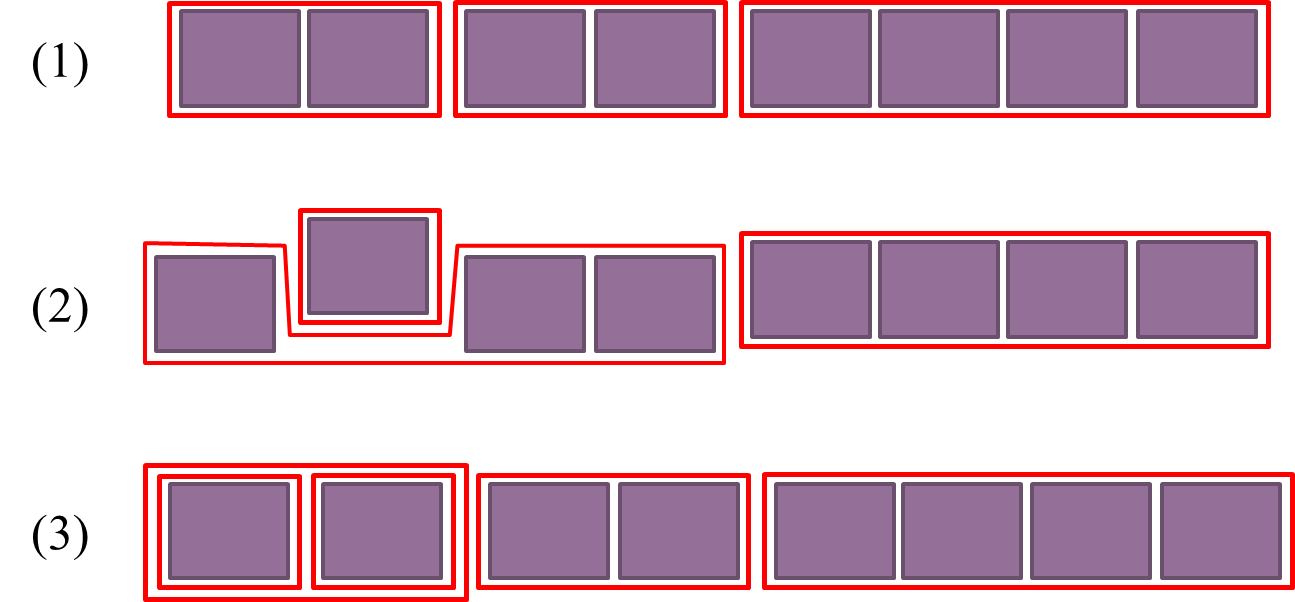
\includegraphics[width=80mm,height=40mm]{slide_segment.png}
 \end{center}
 \caption{セグメント}
 \label{fig:segment}
\end{figure}


\subsubsection{tf-idf によるセグメント分割}

本研究では,tf-idfのスコアを利用した単語ベクトルを生成し,セグメントのコサイン類似度を利用する.
文書集合 $D$ の中の文書 $d$ に含まれる単語 $t$ のtfidfは,$t$の$d$内の出現回数を $tf(t, d)$,
単語$t$が出現する文書の数を $df(t, D)$ とすると,文書dにおける単語tのtfidfは

\begin{equation}
 tfidf(t, d, D) = \frac{tf(t, d)}{df(t, D)}
\end{equation}

とする.

これを用いて,以下の手順でセグメント分割を行う.

\begin{enumerate}
 \item 初期状態として,すべてのセグメントはシート1枚で一つのセグメントとする.
 \item 各セグメントについて,文書の単位をシート一枚とし,\\
$D = (スライドに含まれるすべてのシート)$\\
$d = (対象のシート)$\\
$t = (dに含まれる単語)$\\
 とし,単語のtf-idfスコアを計算し単語ベクトルを生成する.
 \item 隣接するセグメントの単語ベクトルのコサイン類似度を計算する.
 \item コサイン類似度が閾値以上のセグメントのうち,コサイン類似度が最も高い2セグメントを一つのセグメントにまとめる.
 \item 2〜4 を繰り返す.
\end{enumerate}

以上によってセグメントを求める.












\section{講義の対応付け}\label{sec:lecture-sim}

次に,講義同士の対応付けを行う.
ここでは,例えば,京都大学の``画像処理''に対して,東京工業大学の``知的画像処理''のような,内容が似たような講義を取得することを目的とする.
これにより,京都大学の``画像処理''の講義スライドを見て学習していて,分からない箇所が有った場合に,東京工業大学の``知的画像処理''の講義スライドを見てみる,といったことが可能になる.

ここでも単語ベクトルのコサイン類似度を使い講義の類似度を計算する.
まず,各講義の単語ベクトルを計算する.
ここでは,講義に含まれるすべてのスライドの集合をドキュメントdとする.
すべてのドキュメントは取得してきたすべての大学のすべての講義とし,各単語のif-idf値を計算し,講義の単語ベクトルとする.

この単語ベクトルを使い,対象講義と他のすべての講義のコサイン類似度を計算し,閾値以上の講義についてを ``類似講義'' とする.この ``類似講義'' について,後に説明するセグメント間の類似度を計算する.

\begin{comment}

\begin{figure}[tb]
 \begin{center}
  \includegraphics[width=8cm,bb=0 0 598 149]{lecsim.jpg}
 \end{center}
 \caption{講義の対応付け}
 \label{fig:lecsim}
\end{figure}

\end{comment}











\section{セグメントの対応付け}\label{sec:segment-sim}

\ref{sec:lecture-sim}章で求めた類似講義について,セグメント単位でさらに対応付けを求める.

例えば,京都大学の``画像処理''の中にはセグメントA,B,C,... があり,東京工業大学の``知的画像処理''の中にはセグメント a, b, c, ... がある場合に,``Aとcは同じ内容について述べている''といったことを取得することを考える.
これを取得することにより,京都大学の``画像処理''の講義スライドのセグメントAが理解できなかった場合に,東京工業大学の``知的画像処理''の講義スライドのセグメントcを参考にする,といったことが可能になる.

図 \ref{fig:segsim} がセグメントの対応付けの例である.
図のように,1回の講義スライドには複数のセグメントが存在している.
ある2つの内容が,ある講義では同じ講義スライドに含まれている場合もあれば,異なる講義スライドに含まれている場合もある.
また,異なる講義で教える順番が前後している場合があったり,ある講義に含まれている内容が別の内容には含まれていないといったことがあり得る.

ここでも同様にコサイン類似度を計算する.
各セグメントをドキュメントdとする.
すべてのドキュメントは,そのセグメントが含まれる講義の中のすべてのセグメント,又は,すべての大学のすべての講義に含まれるすべてのセグメントとすることを考えている.

\begin{figure}[tb]
 \begin{center}
  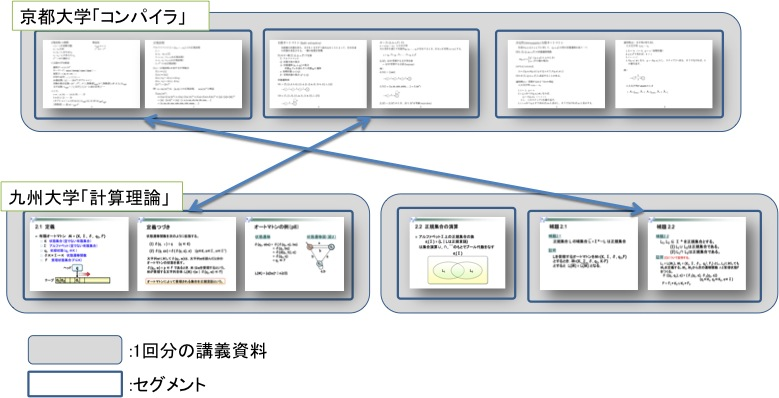
\includegraphics[width=8cm,bb=0 0 779 398]{segsim.jpg}
 \end{center}
 \caption{セグメントの対応付け}
 \label{fig:segsim}
\end{figure}






\section{スライドのわかりやすさ}

本研究では,学習者の理解支援のため,独学しやすいスライドを提示することを考えている.
そのため,以下の尺度から,``わかりやすさ'' を求めることを考えている.

\subsection{スライドの画像とテキストの割合}

スライドには画像が画像が含まれている場合も多い.
しかし,テキストによる記述がなく,画像だけの場合は独学には向いていない.
また,逆にテキストの記述ばかりで画像が無い場合も,学習者にとってわかりやすいスライドとは言えない.
そのため,スライドに含まれるテキストと画像の割合を計算し,ユーザーにとって理解しやすいスライドを提示することを考えている.


\subsection{テキストの記述のわかりやすさ}

スライドのテキストは,文章で記述されている場合と,箇条書きになっている場合がある.
しかし,箇条書きの場合は,独学に向かない場合があると考えられる.
そこで,テキストを形態素解析し,その品詞によって,文章のわかりやすさを評価することも考えられる.





\section{おわりに}

本研究では,スライドをセグメントに分割し,セグメントの対応付けを行うことで,
講義スライドを用いて学習している人への学習支援を行うことを考えた.
今後の課題としては,評価実験についてと,セグメント分割の精度向上,
スライドのわかりやすさ尺度の具体的な提示方法考案などが挙げられる.

評価実験に関しては,現在,セグメントの評価と,スライドのわかりやすさ尺度の評価を行っている.

セグメント分割の精度向上については,スライドの記述料が少なく,うまく分割されないことが問題となっている.
そこで,スライドから専門用語を抽出することで,少ないテキストから重要な情報を活用することを考えている.










% \vspace{30mm}

\begin{thebibliography}{99}


\bibitem{hayama2008}
羽山徹彩, 難波英嗣, 國藤進:
``プレゼンテーションスライド情報の構造化'',
電子情報通信学会技術研究報告, 2008, Vol. 70, pp. 45-50

\bibitem{hayama2009}
羽山徹彩, 難波英嗣, 國藤進:
``プレゼンテーションスライド情報の構造抽出'', 
電子情報通信学会論文誌D, Vol. J92-D(9), pp. 1483-1494, 2009-09

\bibitem{hayama2010}
羽山徹彩, 國藤進: 
``プレゼンテーションスライド情報検索のためのスライドページからの要求関連情報抽出'',
日本情報処理学会研究報告, 2010, DD-76(2)

\bibitem{kitayama2009}
北山大輔, 大谷亜希子, 角谷和俊: 
``プレゼンテーションコンテンツのためのシーン意味的関係抽出とその応用'', 
 情報処理学会論文誌データベース, Vol.2 No.2, pp. 71-85, 2009-06

%\bibitem{wang2010}
%王元元, 北山大輔, 角谷和俊: 
%``プレゼンテーションコンテンツのための概念的構造と表層的構造に基づくスライドの関係判定方式'',
%DEIM Forum, 2010 C1-1

\bibitem{wang201009}
Yuanyuan Wang and Kazutoshi Sumiya: 
``Semantic Ranking of Lecture Slides based on Conceptual Relationship and Presentational Structure'',
1st Workshop on Recommender Systems for Technology Enhanced Learning, pp. 2801-2810, 2010-09

%\bibitem{vinc2006}
%Alessandro Vinciarelli and Jean-Marc Odobez: 
%``Application of Information Retrieval Technologies to Presentation Slides'', 
%IEEE TRANSACTIONS ON MULTIMEDIA, VOL. 8, NO. 5, pp. 981-995, 2006-10

%\bibitem{atapattu2012}
%Thushari Atapattu, Katrina Falkner, Nickolas Falkner:
%``Automated Extraction of Semantic Concepts from Semi-structured Data: Supporting Computer-Based Education through the Analysis of Lecture Notes'',
%Databace and Expert Systems Applications, pp161-175, 2012, 

\bibitem{tanaka2012}
田中清太郎, 手塚太郎, 青山敦, 木村文則, 前田亮: 
``図形の形状と配置に着目したスライド検索手法の提案'',
DEIM Forum, 2012 E6-4

%\bibitem{tomoyasu2012}
%友安航太, 王元元, 角谷和俊:
%``ポスターとスライドの構造に基づくズーミングを用いたポスター閲覧方式'',
%日本情報処理学会研究報告, 2012, DBS-155(1)

% \bibitem{minyen2007}
% Min-yen Kan:
% ``SlideSeer: A digital library of aligned document and presentation pairs'',
% Joint Conference on Digital Libraries, pp. 81-90, 2007

%\bibitem{yamada1999}
%山田卓也, 前野真輝, 渡邉豊英, 佐川雄二:
%``ユーザの意図を反映したシナリオに基づいたプレゼンテーション・スライド構成支援'',
%情報処理学会研究報告, 1999, 99(85)


%\bibitem{sakamoto2013} 坂本祥之, 清水敏之, 吉川正俊:
%``プレゼンテーションスライドからの構成抽出'',
%DEIM2013, D5-4

%\bibitem{tajima1998} Keishi Tajima, Yoshiaki Mizuuchi, Masatsugu Kitagawa:
%``Cut as a Querying Unit for WWW, Netnews, and E-mail'',
%HYPERTEXT, 1998

\bibitem{okamoto2004} 岡本拓明, 小林隆志, 横田治夫:
``プレゼンテーション蓄積検索システムにおける適合度計算の改善'',
DEWS2004, 1-B-03

\bibitem{wang2013} Yuanyuan Wang, Kazutoshi Sumiya:
``Dynamic Word Clouds: Context-based Word Clouds of Presentation Slides for Quick Browsing'',
IIMSS, 2013


\end{thebibliography}


\end{document}
